\section{Tangent lines}

The slope is computed by Lua in the units of the coordinate system, so a tangent line is correct even when \tkzname{xstep} and \tkzname{ystep} are different. Each tangent line is made of two half-lines: on the left (l) and on the right (r). Their lengths are given by \tkzname{kl} and \tkzname{kr}, in units of the $x$-axis: the right half goes from the point of tangency $(a, f(a))$ to the point $(a+k_r, f(a)+k_r f'_+(a))$. With $kl=0$ or $kr=0$, the corresponding half is not drawn.

If the function is not differentiable at $a$, the two halves have different slopes; they are computed separately.

\subsection{Drawing a tangent line: \tkzcname{tkzFnTangent}}

\begin{NewMacroBox}{tkzFnTangent}{\oarg{options}\parg{name of the function,$a$}}
\begin{tabular}{lll}
 \toprule
 arguments             & example & explanation    \\
 \midrule
 \TAline{function,a}{(f,0)}{tangent line at the point with $x=0$}
 \bottomrule
\end{tabular}

\begin{tabular}{lll}
\toprule
options             & default & definition                         \\
\midrule
\TOline{draw}{false}{the point of tangency is drawn}
\TOline{kl}{1}{length of the left half (units of the $x$-axis)}
\TOline{kr}{1}{length of the right half}
\TOline{clip}{true}{the line is clipped to the window}
\bottomrule
\end{tabular}

\emph{Other options are \TIKZ\ options; the style is \tkzname{tkzfn tangent}, empty by default. To get the arrows of \tkzname{tkz-fct}:}

|\tikzset{tkzfn tangent/.style={->,>=latex}}|
\end{NewMacroBox}

\tkzHand The function does not need to be drawn; it only has to be defined.

%<--------------------------------------------------------------------------->
\subsection{Tangent line when \tkzname{xstep} and \tkzname{ystep} are not 1}

No computation is needed: just use the values of the tick marks.

\begin{tkzexample}[vbox]
\begin{tikzpicture}[xscale=1.5]
 \tkzFnInit[xmin=0,xmax=800,xstep=100,
            ymin=0,ymax=1800,ystep=400]
 \tkzFnGrid[color=brown,sub,subdx=50,subdy=200](0,0)(800,1800)
 \tkzFnAxes
 \tkzFnDraw[name=f,color=red,samples=100,domain=0:800]
    {(1/90000)*x^3-(1/100)*x^2+(113/36)*x}
 \tkzFnTangent[draw,color=blue,kr=300,kl=450](f,450)
 \tkzFnText[draw,color=black,fill=brown!50,opacity=0.8](300,1200)
 {$f(x)=\dfrac{1}{90000}x^3 -\dfrac{1}{{100}}x^2 +\dfrac{113}{36}x$}
\end{tikzpicture}
\end{tkzexample}

The slope at $450$ is $\tkzFnPrint[4]{diff(f,450)}$; it is obtained with |\tkzFnPrint[4]{diff(f,450)}|.

%<--------------------------------------------------------------------------->
\subsection{The options \tkzname{kl}, \tkzname{kr} and \tkzname{draw}}

\begin{tkzexample}[]
\begin{tikzpicture}[scale=1.5]
  \tikzset{tkzfn tangent/.style={->,>=latex}}
  \tkzFnInit[xmin=-3,xmax=4,ymin=-4,ymax=2]
  \tkzFnGrid  \tkzFnAxes[ticks=false]
  \tkzFnDraw[name=f,domain=-2.15:3.2]{-x*x+2*x}
  \tkzFnDefPoint[draw](f,2){A}
  \tkzFnTangent[kl=0,draw](f,-1)
  \tkzFnTangent[draw](f,1)
  \tkzFnTangent[kr=0,draw](f,3)
  \tkzFnRep
\end{tikzpicture}
\end{tkzexample}

%<--------------------------------------------------------------------------->
\subsection{Tangent line with two functions}
The option \tkzname{with} of \tkzname{tkz-fct} no longer exists: the function is given by its name.

\begin{tkzexample}[]
\begin{tikzpicture}[scale=4]
 \tkzFnInit[xmin=0,xmax=3,ymin=0,ymax=2]
 \tkzFnAxes
 \tkzFnGrid(0,0)(3,2)
 \tkzFnDraw[name=f,color=red,domain=1/3:3]
           {0.125*(3*x-1)+0.375*(3*x-1)/(x*x)}
 \tkzFnDraw[name=g,color=blue,domain=1/3:3]
           {0.125*(3*x-1)}
 \tkzFnTangent[color=blue](f,1)
 \tkzFnText[draw,color=red](1,1.5)
   {$f(x)=\frac{1}{8}(3x-1)+\frac{3}{8}\left(\frac{3x-1}{x^2}\right)$}
 \tkzFnText[draw,color=blue](2,0.3)
   {$g(x)=\frac{1}{8}(3x-1)$}
\end{tikzpicture}
\end{tkzexample}

%<--------------------------------------------------------------------------->
\subsection{A few tangent lines}

\begin{tkzexample}[]
\begin{tikzpicture}[scale=2]
  \tkzFnInit[xmin=-5,xmax=2,ymin=-1,ymax=3]
  \tkzFnAxes[ticks=false]
  \tkzFnText[draw,color=red,fill=orange!20](1.5,1.5){$y = xe^x$}
  \tkzFnDraw[name=f,color=red,domain=-5:1]{x*exp(x)}
  \tkzFnTangent[color=blue,kr=2,kl=2](f,-2)
  \tkzFnTangent[color=green,kr=2,kl=2](f,-1)
  \tkzFnTangent[color=blue](f,0)
  \tkzFnTangent[color=blue,kr=0](f,1)
\end{tikzpicture}
\end{tkzexample}

%<--------------------------------------------------------------------------->
\subsection{One-sided tangent lines}
At $0$, the function $f$ defined by $f(x)=\sqrt{x^3+x^2}$ is not differentiable: the two halves are obtained automatically.

\begin{tkzexample}[]
 \begin{tikzpicture}[scale=2.75]
     \tkzFnInit[xmin=-2,xmax=3,ymin=0,ymax=3]
     \tkzFnGrid[color=orange](-2,0)(3,3)
     \tkzFnAxes
     \tkzFnDraw[name=f,color=red,domain=-1:2]{sqrt(x^3+x^2)}
     \tkzFnTangent(f,0)
     \tkzFnText[draw,color=red,fill=orange!20](2,1){$f(x)=\sqrt{x^3+x^2}$}
 \end{tikzpicture}
\end{tkzexample}

%<--------------------------------------------------------------------------->
\subsection{One-sided tangent lines: Lorenz curve}

Here only the halves between 0 and 1 are wanted: give the value 0 to \tkzname{kl} in one case and to \tkzname{kr} in the other.

\begin{center}
\begin{tkzexample}[vbox]
\begin{tikzpicture}[scale=1.25]
  \tkzFnInit[xmin=0,xmax=1,ymin=0,ymax=1,xstep=0.1,ystep=0.1]
  \tkzFnGrid(0,0)(1,1)
  \tkzFnAxes
  \tkzFnDraw[name=f,color=red,thick,domain=0:1]{(exp(x)-1)/(exp(1)-1)}
  \tkzFnTangent[draw,kl=0,  kr=0.4](f,0)
  \tkzFnTangent[draw,kl=0.4,kr=0  ](f,1)
  \tkzFnText[draw,color=red,fill=orange!20](0.5,0.6)
          {$f(x)=\dfrac{\text{e}^x-1}{\text{e}-1}$}
\end{tikzpicture}
\end{tkzexample}
\end{center}

%<--------------------------------------------------------------------------->
\subsection{A family of tangent lines}

Tangent lines can be drawn in a \tkzcname{foreach} loop.

\begin{tkzexample}[vbox]
\begin{tikzpicture}[scale=2]
  \tkzFnInit[xmin=-5,xmax=2,ymin=-1,ymax=3]
  \tkzFnAxes[ticks=false]
  \tkzFnText[draw,color=red,fill=orange!20](1.5,1.5){$y = xe^x$}
  \tkzFnDraw[name=f,line width=0.01pt,color=red,domain=-5:1]{x*exp(x)}
  \foreach \v in {-4,-3.8,...,0}{
    \tkzFnTangent[color=blue,line width=.4pt,kr=1,kl=0.5](f,\v)}
  \foreach \v in {0.6,0.8,1}{
    \tkzFnTangent[color=blue,line width=.4pt,kr=0,kl=0.5](f,\v)}
\end{tikzpicture}
\end{tkzexample}

%<--------------------------------------------------------------------------->
\subsection{Tangent lines without the curve}

The function is defined with \tkzcname{tkzFnDef} but not drawn.

\begin{tkzexample}[vbox]
\begin{tikzpicture}[scale=2]
  \tkzFnInit[xmin=-5,xmax=2,ymin=-1,ymax=3]
  \tkzFnAxes[ticks=false]
  \tkzFnText[draw,color=red,fill=orange!20](1.5,1.5){$y = xe^x$}
  \tkzFnDef{f}{x*exp(x)}
  \foreach \v in {-4,-3.8,...,0}{
    \tkzFnTangent[color=blue,line width=.4pt,kl=1](f,\v)}
  \foreach \v in {0.6,0.8,1}{
    \tkzFnTangent[color=blue,line width=.4pt,kr=0,kl=.75](f,\v)}
\end{tikzpicture}
\end{tkzexample}

\newpage
\subsection{Point of tangency given by an expression}

The $x$-coordinate of the point of tangency can be a Lua expression; if it contains parentheses, put it between braces.

\begin{center}
\begin{tkzexample}[]
\begin{tikzpicture}[scale=1]
  \tkzFnInit[xmin=0,xmax=1,xstep=0.1,
             ymin=0.5,ymax=1,ystep=0.1]
  \tkzFnGrid \tkzFnAxes
  \tkzFnDraw[name=f,domain=0.00001:1]{x^x}
  \tkzFnTangent[draw,color=red,kr=0.2,kl=0.2](f,{1/exp(1)})
\end{tikzpicture}
\end{tkzexample}
\end{center}

\endinput
